\documentclass[11pt]{article}
\usepackage[margin=1.5in]{geometry}
\usepackage{graphicx}
\usepackage{float}
\usepackage{parskip}
\usepackage{amsmath}
\usepackage{subfigure}
\usepackage{ulem}
\usepackage{pgfplots}
\usepgfplotslibrary{polar}
\pgfplotsset{width=10cm, compat=1.9}

\begin{document}

\textbf{\Huge Conics}

Athan Zhang \& Jeffrey Chen

\section{Introduction to Conic Sections}

Conic sections, simply called \textbf{conics}, are figures formed when a plane intersects a double-napped right cone (two cones opposite each other and extending infinitely upward and downward). 

\begin{figure}[H]
    \centering
    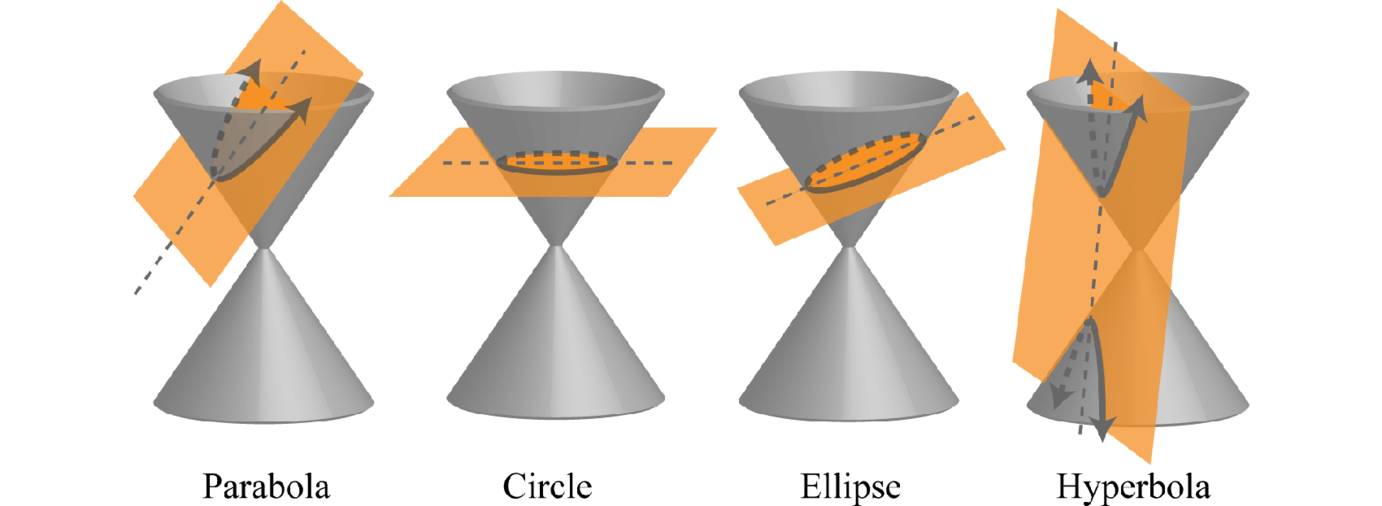
\includegraphics[width=0.9\textwidth]{Precalc/images/conic_sections.png}
\end{figure}

The above graphic shows the four most common types of conics. As we can see, these are all types of equations we've learned about before. They are the parabola, ellipse, circle, and hyperbola.

In a special case where the plane intersects the vertex of the cone, the figures formed are called \textbf{degenerate conics}. This includes a singular point, a line, or two intersecting lines.

The general form of the equations for conic sections if
\begin{align*}
    Ax^2 + Bxy + Cy^2 + Dx + Ey + F = 0
\end{align*}
where $A$, $B$, and $C$ cannot all be zero. As we continue on in this chapter, more specific algebraic forms for each conic will be addressed.

\section{Parabola}

A \textbf{locus} is a set of all points that fulfill a geometric property. A \textbf{parabola} represents the locus of points in a plane that are equidistant from a fixed point, called the \textbf{focus} and a specific line, called the \textbf{directrix}. Furthermore, a parabola is symmetric about the line perpendicular to the directrix through the focus called the \textbf{axis of symmetry}. The \textbf{vertex} is the intersection of the parabola and the axis of symmetry and is usually the tip of the parabola.

Let $P(x,y)$ be any point on the parabola. Let $p$ be the distance from the vertex to the focus. By the definition of a parabola, the distance from any point on the parabola to the focus must equal the distance from that point to the directrix. So, we know that $p$ is also the distance from the point to the directrix. If we write the vertex as $(h, k)$, we know that the coordinate of a point on the directrix is $(h - p, y)$, assuming it is a horizontal parabola.

We can use the distance formula to determine the equation for the parabola.

\begin{align*}
    p &= p \\
    \sqrt{[x - (h+p)]^2 + (y - k)^2} &= \sqrt{[x - (h - p)]^2 + (y-y)^2} \\
    [x - (h + p)]^2 + (y-k)^2 &= [x - (h-p)]^2 + 0^2 \\
    x^2 - 2x(h+p) + (h+p)^2 + (y-k)^2 &= x^2 - 2x(h-p) + (h-p)^2 \\
    x^2 - 2xh - 2xp + h^2 + 2hp + p^2 + (y-k)^2 &= x^2 -2xh + 2xp + h^2 - 2hp + p^2 \\
    (y-k)^2 &= 4xp - 4hp \\
    (y-k)^2 &= 4p(x - h)
\end{align*}

An equation for a parabola that opens horizontally is thus given as $(y-k)^2 = 4p(x - h)$. Similarly, for parabolas that open vertically, we can derive a similar equation in which we switch $x$ and $y$, giving $(x-h)^2 = 4p(y - x)$.

\textbf{Key Properties}
\begin{enumerate}
    \item The focus and directrix will be a distance $p$ above and below the vertex, respectively, depending on horizontal or vertical orientation.
    \item The distance $p$ can be calculated from the form $(y-k)^2 = 4p(x - h)$ or $(x-h)^2 = 4p(y - x)$.
    \item The Latus rectum is a line segment of length $4p$ and is parallel to the directrix and passes through the focus. 
    \item A line $\ell$ that is tangent to a parabola at a point $P$ forms an isosceles triangle such that the segment from $P$ to the focus forms one leg of the triangle and that another segment of the same length lies along the axis of symmetry,
\end{enumerate}

An interesting property is that any ray will reflect the focus. This is why some satellite dishes use parabolic shapes, as electromagnetic signals will be reflected to a singular point on the dish. 

\section{Ellipses and Circles}

An ellipse is the locus of points in a plane such that the sum of the distances from two fixed points, called \textbf{loci}, is constant. To visualize this concept, we can consider a piece of string tied around two thumbtacks on a board. If we trace a curve with the string being pulled tight, we will have an ellipse. 

A line segment containing an ellipse's foci and endpoints on the ellipse is called the \textbf{major axis}, and the midpoint of the major axis is \textbf{center}. The major axis is usually the widest part of the eclipse. The segment through the center with endpoints on the ellipse and perpendicular to the major axis is called \textbf{minor axis}. The two endpoints of the major axis are the \textbf{vertices}, and the endpoints of the minor axis are the \textbf{co-vertices}.

Let $P(x,y)$ be any point on the ellipse with center $C(h,k)$. By the definition of an ellipse, the sum of distances from any point on the ellipse to the foci is constant and should equal the length of the major axis. This length is given as $2a$, where $a$ is the length of the semi-major axis is the distance from the center to a vertex.

{\tiny 
\begin{align*}
    \sqrt{[x - (h-c)]^2 + (y-k)^2} + \sqrt{[x-(h+c)]^2 + (y-k)^2} &= 2a \\
    \sqrt{[x - h + c]^2 + (y-k)^2} &= 2a - \sqrt{[x - h - c)]^2 + (y-k)^2} \\
    \sqrt{[(x-h) + c]^2 + (y-k)^2} &= 2a - \sqrt{[(x - h) - c]^2 + (y-k)^2} \\
    [(x-h) + c]^2 + (y-k)^2 &= 4a^2 - 4a\sqrt{[(x - h) - c]^2 + (y-k)^2} + [(x - h) - c]^2 + (y-k)^2 \\
    (x-h)^2 + 2c(x-h) + c^2 + (y-k)^2 &= 4a^2 - 4a\sqrt{[(x - h) - c]^2 + (y-k)^2} + (x-h)^2 - 2c(x-h) + c^2 + (y-k)^2 \\
    4a\sqrt{[(x - h) - c]^2 + (y-k)^2} &= 4a^2 - 4c(x-h) \\
    a\sqrt{[(x - h) - c]^2 + (y-k)^2} &= a^2 - c(x-h) \\
    a^2[(x-h)^2 - 2c(x-h) + c^2 + (y-k)^2] &= a^4 - 2a^2 c(x-h) + c^2 (x-h)^2 \\
    a^2(x-h)^2 - 2a^2c(x-h) + a^2 c^2 + a^2(y-k)^2 &= a^4 - 2a^2 c(x-h) + c^2 (x-h)^2 \\
    a^2(x-h)^2 - c^2(x-h)^2 + a^2(y-k)^2 &= a^4 - a^2 c^2 \\
    (a^2 - c^2)(x-h)^2 + a^2(y-k)^2 &= a^2(a^2 -c^2) \\
    b^2 (x-h)^2 + a^2(y-k)^2 &= a^2 b^2 \\
    \frac{(x-h)^2}{a^2} + \frac{(y-k)^2}{b^2} &= 1\\
\end{align*}
}%

The standard form for an ellipse centered at $(h,k)$, where $a > b$ is given as
\begin{align*}
    \frac{(x-h)^2}{a^2} + \frac{(y-k)^2}{b^2} = 1
\end{align*}
Keep in mind that this is the form of the ellipse that has a horizontal major axis. If it has a vertical major axis, the form is
\begin{align*}
    \frac{(x-h)^2}{b^2} + \frac{(y-k)^2}{a^2} = 1
\end{align*}

The \textbf{eccentricity} of an ellipse is the ratio of $c$ to $a$. This value will always be between 0 and 1 and will determine how circular the ellipse will be. If $e = 0$, we know that $c = 0$, which means both foci are at the center, making it a  circle. When $e = 1$, we know that $c = a$, which means the foci are at the vertices.

\section{Hyperbolas}

A hyperbola is the locus of all points in a plane such that the absolute value of the differences in the distances between two foci is constant.  

The graph of a hyperbola consists of two disconnected branches that approach two asymptotes. The midpoint of the segment with endpoints at the foci is the center. The vertices are at the intersection of this segment and each branch of the curve. Like an ellipse, a hyperbola has two axes of symmetry. The \textbf{transverse axis} has a length of $2a$ units and connects the vertices. The \textbf{conjugate axis} is perpendicular to the transverse, passes through the center, and has a length of $2b$ units. 

The relationship among the values of $a$, $b$, and $c$ is different for a hyperbola than it is for an ellipse. For a hyperbola, the relationship is $c^2 = a^2 + b^2$ whereas it was $a^2 = b^2 + c^2$ in an ellipse. The proof for the standard form of a hyperbola is similar to an ellipse, however, we subtract the distances instead of adding. This yields the following form for a hyperbola centered at $(h,k)$.
\begin{align*}
    \frac{(x-h)^2}{a^2} - \frac{(y-k)^2}{b^2} = 1
\end{align*}
Keep in mind that this is the form of the hyperbola that has a horizontal transverse axis. If it has a vertical transverse axis, the form is
\begin{align*}
    \frac{(y-k)^2}{a^2} - \frac{(x-h)^2}{b^2} = 1
\end{align*}

\section{Identifying Conic Sections}

We know that the conic is in the general form of $Ax^2 + Bxy + Cy^2 + Dx + Ey + F = 0$. The discriminant, or $B^2 - 4AC$, can be used to identify the conic.
\begin{itemize}
    \item Circle if $B^2 - 4AC < 0$; $B = 0$ and $A = C$
    \item Ellipse if $B^2 - 4AC < 0$; either $B \neq 0$ or $A \neq C$
    \item Parabola if $B^2 - 4AC = 0$
    \item Hyperbola if $B^2 - 4AC > 0$
\end{itemize}

When $B = 0$, the conic will either be vertical or horizontal. When $B \neq 0$, the conic will be neither vertical nor horizontal.

\end{document}